\documentclass{article}

\usepackage[final]{neurips_2024}
\usepackage{amsmath}
\usepackage{graphicx}
\usepackage{algorithm}

\usepackage[utf8]{inputenc} % allow utf-8 input
\usepackage[T1]{fontenc}    % use 8-bit T1 fonts
\usepackage{hyperref}       % hyperlinks
\usepackage{url}            % simple URL typesetting
\usepackage{booktabs}       % professional-quality tables
\usepackage{amsfonts}       % blackboard math symbols
\usepackage{nicefrac}       % compact symbols for 1/2, etc.
\usepackage{microtype}      % microtypography
\usepackage{xcolor}         % colors

\title{Pop Stars Have Something to Teach CU Professors: \\
\large{How Low Can You Go with Sentence Embeddings to Stay Useful?}}

\begin{document}

\author{%
  Alena Chan \\
  Department of Computer Science \\
  Columbia University \\
  New York, USA \\
  \texttt{ac5477@columbia.edu} \\
  \And
  Aksel Kretsinger-Walters \\
  Department of Computer Science \\
  Columbia University \\
  New York, USA \\
  \texttt{adk2164@columbia.edu} \\
  \And
  Maria Garmonina \\
  Department of Applied Mathematics \\
  Columbia University \\
  New York, USA \\
  \texttt{mkg2169@columbia.edu} \\
}

\maketitle

\begin{abstract}
		\textit{How much embedding dimensionality is needed for a given corpus? Can a model
		trained on a simpler domain transfer effectively to semantically richer tasks?}

		To answer these questions, we study how domain and embedding dimensionality interact in
		unsupervised sentence encoders. Using two extreme corpora, \textbf{Taylor Swift lyrics
		and Nakul Verma's papers}, we train \textbf{contrastive BERT models from 4D to 767D}
		and evaluate geometry and transfer learning properties.

		Surprisingly, lower-dimensional \textbf{models trained on lyrics (4–256D) outperform
		paper-trained models on STS-B}, with papers only catching up at 767D. This suggests
		that simple, high-frequency text can be an efficient pretraining source for compact
		encoders, while complex text needs far more dimensions to expose useful structure.
\end{abstract}

\section{Introduction}
% Recently there have been much progress in improving quality of sentence embeddings, like BERT[cite] family of models. However, training such requires vast amounts of data (billions of words for BERT), and these embeddings are later used per se. BERT embeddings are either used, as is, in 768D, or target dimension is determined by memory or compute limits. \\
% Efficient embedding is determined by data in question, here it is natural that different "topics" and "concepts" would be best represented through different maps. \\
% We consider how much subspace of English sentences related to two chosen topics (\textit{pop songs} and \textit{scientific papers}) capture semantic relations pertaining to general English, and how much knowledge about structure of one subspace transfers to the other. In addition, we explore intrinsic dimensionality of these subspaces. \\
% To validate our findings we compare performance of embedding transfer across tasks. We apply two-step training method for sentence representation learning models. \\
% We introduce tools for future evaluation of concept-dimensionality. To propose metrics to analyze efficiency of topic embeddings, in terms of capturing semantic meaning and ability to transfer to general language. We also give practical way to split text into meaningful units and assign similarity in self-supervised way. \\
% Efficient embedding is a function of both raw data and target task. We evaluate embeddings on sematic similarity task as it is fundamental to NLP, and has long been used as training objective in language models and as language comprehension metrics. % citation?
% What concepts allows for smaller-dimensional representations to still capture meaning? How sensitive is representation quality slightly suboptimal dimensionality for each concept?
Sentence embeddings are mappings from high-dimensional linguistic signals to lower-dimensional structures whose geometry captures the semantic meanings of sentences. Latent space embeddings are crucial in NLP tasks. Recent progress—including the BERT [cite] family of models—has significantly improved sentence embedding quality. However, training these models requires vast amounts of data (billions of words for BERT), and the resulting embeddings are typically used as-is. In practice, BERT embeddings are either retained in their original 768-dimensional form or reduced only according to memory or compute constraints.
Yet efficient embedding dimensionality is determined not merely by model architecture but also by the nature of the data itself. Different topics and conceptual domains may naturally admit representations that lie in different effective subspaces.
We investigate how much the subspaces associated with two distinct English domains—pop songs and scientific papers—capture semantic relations relevant to general English, and to what extent structural information learned in one subspace transfers to the other. In addition, we examine the intrinsic dimensionality of these topic-specific subspaces.
To validate our findings, we compare task performance under various forms of embedding transfer. We train sentence representation models using a two-step procedure and evaluate their ability to generalize across domains.
We also introduce tools for future evaluation of concept-dimensionality. Our goal is to provide metrics for analyzing the efficiency of topic-specific embeddings in terms of how well they capture semantic meaning and how effectively they transfer to broader language understanding. Moreover, we propose a practical method for segmenting text into meaningful units and assigning semantic similarity in a self-supervised manner.

Efficient embedding dimensionality is a function of both the raw data and the target task. We evaluate embeddings on a semantic similarity task, as it is foundational in NLP and has long served both as a training objective for language models and as a measure of language comprehension.

This raises two central questions: Which conceptual domains allow for smaller-dimensional representations that still capture meaning? And how sensitive is representation quality to slight deviations from the optimal dimensionality for each concept?

\subsection{Related Work}
Recent work on sentence embeddings has focused on understanding and improving the
geometry of representation spaces. I'll briefly summarize the papers we referenced as we
brainstormed and implemented our project.

Wang \& Isola (2020) \cite{wang2020contrastive} demonstrate that contrastive learning optimizes two
competing objectives—alignment of similar examples and uniformity of representations on
the hypersphere—providing a geometric framework that underlies many modern embedding
methods. Gao et al. (2021) \cite{gao2021simcse} introduce SimCSE, showing that simple
dropout-based positive pairs produce state-of-the-art unsupervised sentence embeddings,
with supervised variants further improving semantic similarity performance. Reimers \&
Gurevych (2019) \cite{reimers2019sentencebert} propose Sentence-BERT, a siamese BERT
architecture enabling efficient cosine-similarity–based retrieval and establishing a
strong benchmark for supervised semantic embedding tasks.

Li et al. (2020) \cite{li2020sentenceembeddingdim} investigate the intrinsic
dimensionality of contextual embeddings, finding strong anisotropy and proposing
geometric corrections to improve isotropy and downstream performance. Wang \& Liu (2021)
\cite{wang2021divergence} analyze the divergence properties of InfoNCE-style losses,
explaining how different contrastive objectives induce distinct geometric structures in
embedding space. Chen et al. (2020) \cite{chen2020simclr} introduce SimCLR, a
vision-based contrastive framework whose insights—especially the role of augmentations
and projection heads—directly inspired modern sentence-level contrastive methods. Amit et
al. (2021) \cite{amit2021intrinsicdim} tie generalization performance to intrinsic
dimensionality, suggesting that models adapt their effective dimensionality to task
complexity. Finally, Hu et al. (2023) \cite{ma2023lora} present LoRA, showing that
learned low-rank subspaces can efficiently adapt large language models—reinforcing the
broader theme that meaningful linguistic structure often lies in low-dimensional manifolds.
\section{Methodology}
We use contrastive learning described in SimCSE [cite]. SimCSE's training objective is to pull positive pairs together in embedding space, and push negative pairs apart. In our context, positive and negative pairs are defined by closeness in the same text, creating self-supervised setting. SimCSE was previously shown successful on STS benchmarks and transfer tasks, which is why we use it as a main semantic meaning learning method. \\
We training two architectures: encoder + pooler (BERT + feed-foward NN), encoder + projection (BERT + PCA).
\subsection{Encoder + pooler}
Here we briefly discuss implementation details, and all code is available. \\
The encoder maps tokens to latent representations, and we use BERT for that.\\
The pooler maps hidden states to low-dimensional embedding of sentences. \\
In [cite], Wang et al. found that performance loss can be decomposed into separate encoder and pooler contributions, which is why we use two-step training procedure. First, we freeze parameters of pooler and fine-tune the encoder, achieving best version of BERT for this dataset; then, we freeze the encoder and train only pooler. This allows to reduce encoder loss and pooler loss sequentially. \\
We load 'bert-base-uncased' weights from Hugging Face for encoder [cite], and construct a fully connected network with $hidden_size x hidden_size$ layer, tanh activation, $hidden_size x projection_size$ fully-connected layer (following Wang et al.). We apply mean pooling to aggregate token embeddings into sentences embeddings; note that BERT porduces position-aware token representations, so orderial information is not lost.\\ %@article{DBLP:journals/corr/abs-1810-04805,
%   author    = {Jacob Devlin and
%                Ming{-}Wei Chang and
%                Kenton Lee and
%                Kristina Toutanova},
%   title     = {{BERT:} Pre-training of Deep Bidirectional Transformers for Language
%                Understanding},
%   journal   = {CoRR},
%   volume    = {abs/1810.04805},
%   year      = {2018},
%   url       = {http://arxiv.org/abs/1810.04805},
%   archivePrefix = {arXiv},
%   eprint    = {1810.04805},
%   timestamp = {Tue, 30 Oct 2018 20:39:56 +0100},
%   biburl    = {https://dblp.org/rec/journals/corr/abs-1810-04805.bib},
%   bibsource = {dblp computer science bibliography, https://dblp.org}
% }
%
We train embeddings as follows. We apply SimCSE trick: a sentence passed as it and with dropout should have similar embeddings. For each anchor sentence, we find multipositive Normalized Temperature-scaled Cross-Entropy loss and optimize using Adam. \\
\subsection{Encoder + projection}
Encoder is BERT followed by PCA.

\subsection{Base model}
\texttt{BERT-base-uncased} with mean pooling. A projection head maps pooled
representations to a target dimension $d \in \{4,16,64,256,767\}$ followed by $L_2$ normalization.

\begin{figure}[h!]
		\centering
		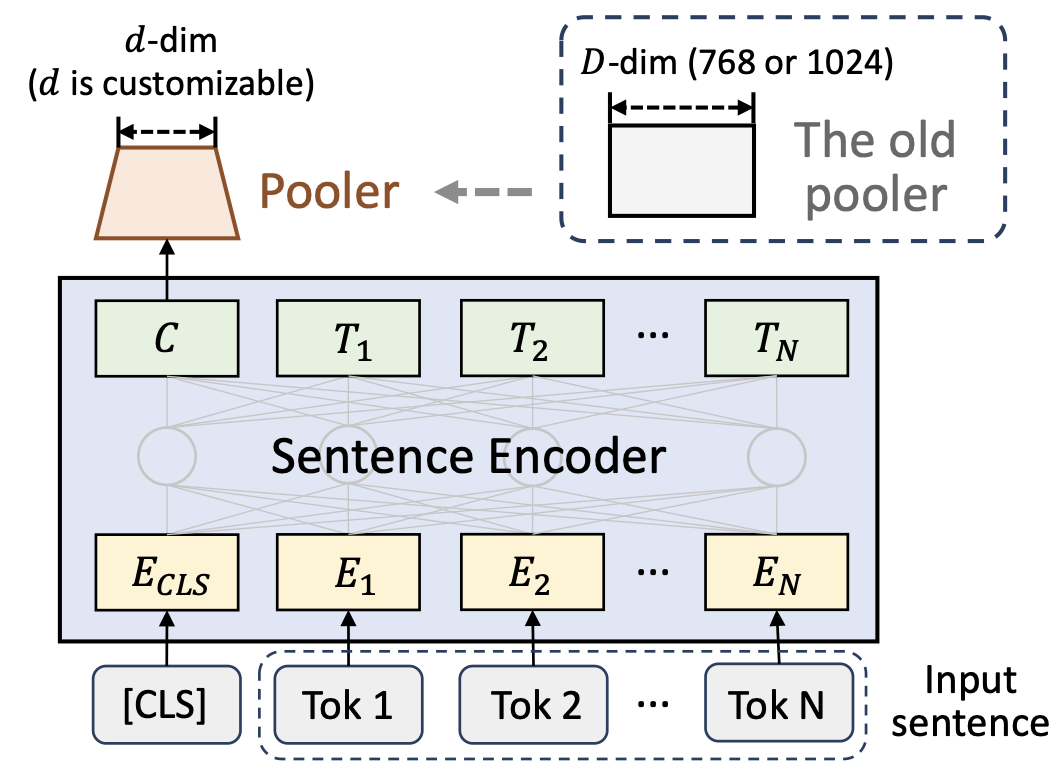
\includegraphics[width=0.6\linewidth]{Images/bert_pooler.png}
		\caption{BERT+Pooler architecture. Image credit: https://arxiv.org/pdf/2310.15285.}
		\label{fig:model_arch}
\end{figure}

\subsection{Training domains}
TODO: add why we choose these domains: to capture different styles + complexity + mode of communication; given drastically opposite fields, ability to capture indicates strong ability to generalize accross language tasks.\\

Each song and each paper section is treated as one document, and neighboring sentences
within a document form positive pairs. The corpora are token-matched for training compute parity:

1) Taylor Swift lyrics (short, repetitive, low-entropy)

2) Nakul Verma's ML papers (long, information-dense)

\subsection{Data preprocessing}

TODO: explain why we look at sentence, not word level - bc semantically meaningful unit is sentence. possibly discuss how sentence notion is funky for songs. \\

Downloading, cleaning, and formatting the datasets into sentence-level documents was a multistep process.

For the lyrics dataset, there was a kaggle repository containing the entire Taylor Swift discography, which we used for our lyrics corpus. The cleanup included removing sequential duplicate sentences, filtering out song and album metadata, and splitting the lyrics into individual sentences using the NLTK sentence tokenizer.

For the papers dataset, we used the arXiv API to download Nakul Verma's papers in pure latex form. There was substantial cleaning and processing work involved from that point. First, we removed latex commands, equations, figures, tables, and references using regex patterns. Next, we split the cleaned text into sentences. These two actions required a fair amount of user judgement, and dimished the size of the usable corpus. \\

Given two corpora, we create pairs of similar sentences in self-supervised manner through assigning similarity indicator based on sentence distance.

\subsection{Training objective}
We train unsupervised SimCSE-style contrastive models with multiple positive examples,
sampling local neighbors within each document. Following Wang et al., 2023
\cite{wang2023}, we use a two-step training scheme:

Step 1. Freeze pooler, train encoder (3 epochs).

Step 2. Freeze encoder, train pooler (3 epochs).

\subsection{Evaluations}

\begin{itemize}
\item Geometry
\begin{itemize}
		\item Alignment and uniformity losses (Wang et al., 2020, \cite{wang2020contrastive}) on in-domain
				and out-of-domain test sets. Alignment measures how close positive pairs are, and
				uniformity captures how evenly embeddings are spread on the hypersphere.
		\item t-SNE embeddings of sentences from songs and papers.
\end{itemize}
\item Transfer learning: STS-B Spearman rank correlations of sentence pair embeddings.
\end{itemize}

\textbf{PCA} projections of the frozen BERT encoder at the same target dimensions are
used as a baseline.

\section{Results and Analysis}

\subsection{Spearman Rank on STS-B}
The results on lyrics-trained models rise sharply between 4D and 256D, peaking long
before the full BERT size of 768D (see Fig. \ref{fig:stsb}). Paper-trained models, in
contrast, only come to full potential at 767D, hinting at a much \textbf{higher intrinsic
dimensionality of scientific text}. Since STS-B is out-of-distribution for both training
corpora, the gap between the performance of songs- and papers-trained models cannot be
attributed to lyrics being much "closer" to STS-B than papers. Instead, it reflects how
contrastive fine-tuning under a low-dimensional bottleneck \textbf{reallocates capacity
of the model}.

On the lyrics corpus, the contrastive task is relatively simple and repetitive, so the
model can solve it without drastically reshaping the pre-trained BERT geometry. A small
projection head is enough to compress lyrics-specific structure while preserving generic
semantic directions that still transfer to STS-B.

On the papers corpus, the contrastive task is much harder: the model must separate dense,
technical sentences within and across sections. In low dimensions, the encoder and head
are forced to specialize for fine-grained distinctions, which distorts general-purpose
semantics and hurts STS-B transfer. Only when we increase the projection size up to
256-767D does the paper-trained model regain enough capacity to encode both in-domain
nuance and broad semantic structure, at which point it overtakes the lyrics-trained model.

The PCA baseline stays near zero Spearman rank across all projection sizes, suggesting
that \textbf{linear compression alone cannot expose semantic structure} -- the pooler must learn it.

\begin{figure}[h!]
\centering
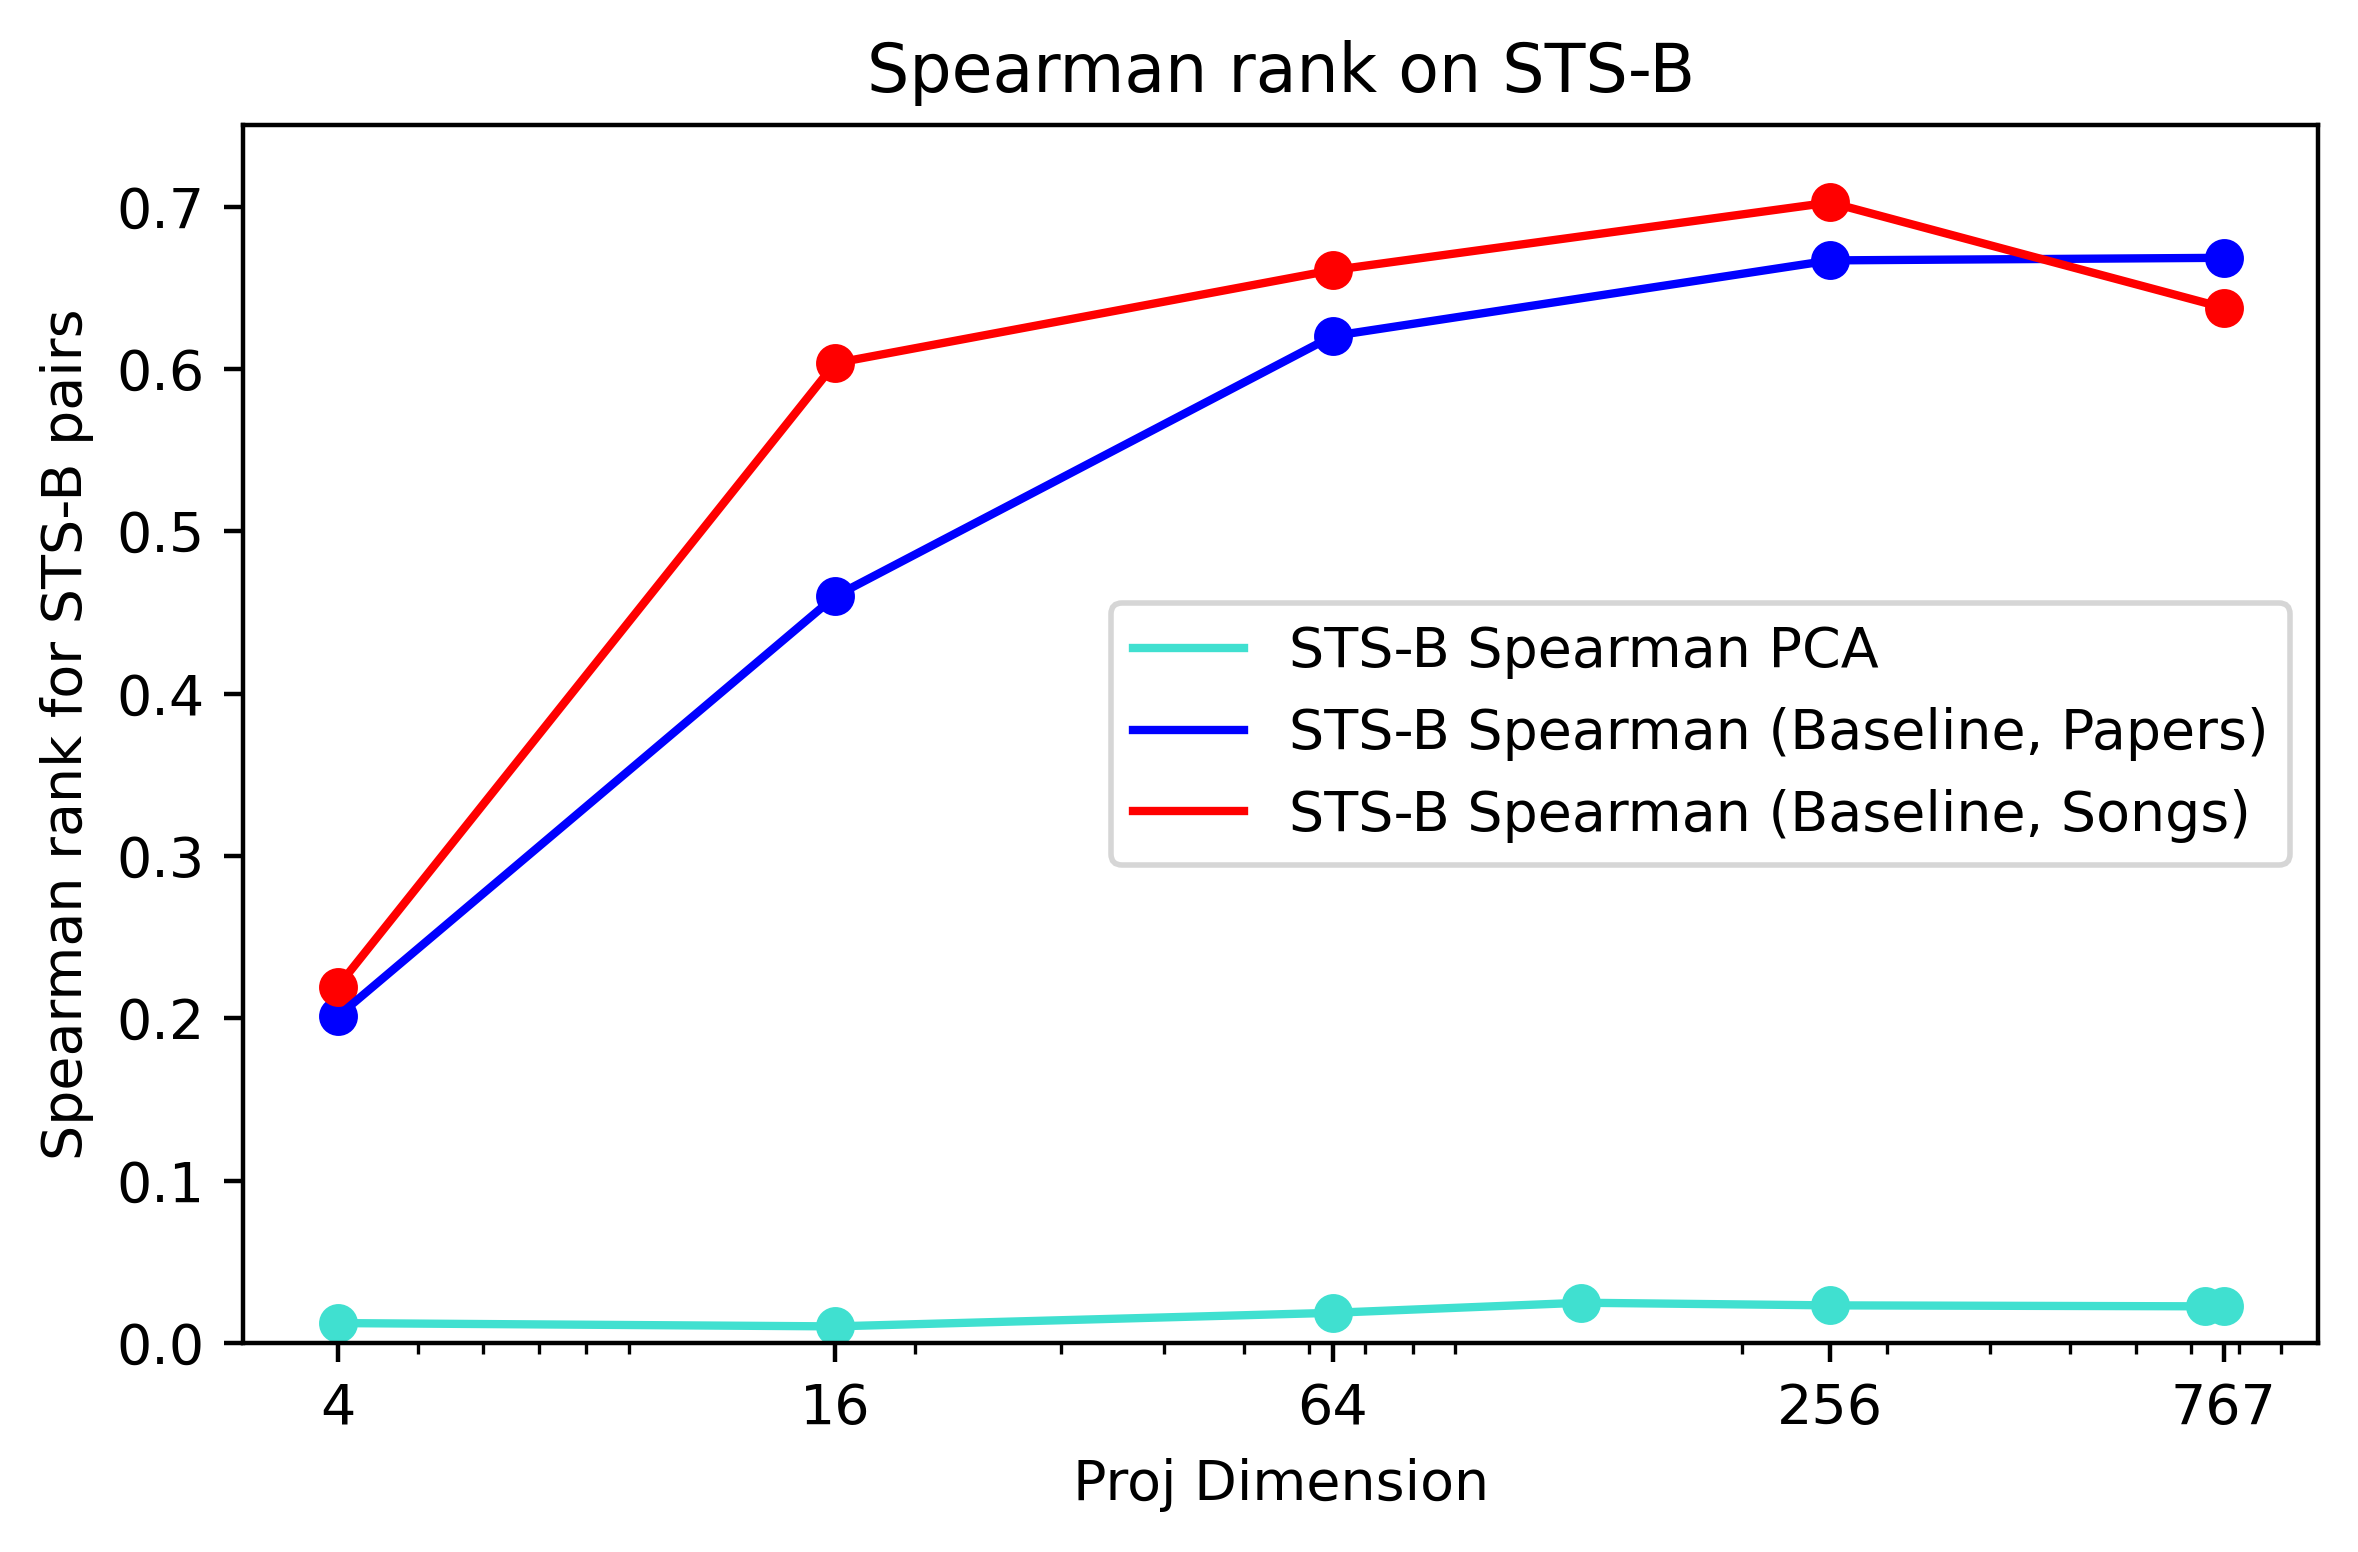
\includegraphics[width=0.6\linewidth]{Images/sts_w_alena.png}
\caption{Spearman rank correlations for BERT+pooler and BERT+PCA variants.}
\label{fig:stsb}
\end{figure}

\subsection{Uniformity and Alignment}
All plots \ref{fig:losses} show the \textbf{alignment vs uniformity tradeoff}: higher
dimensions improve uniformity but degrade alignment. For PCA specifically, uniformity
losses are much smaller than alignment losses for all dimensions, indicating that
embedded sentences occupy the full hypersphere but do not preserve local similarity structure.

For contrastive training, \textbf{in-domain data} (eg. songs embedded with a model
trained on songs) \textbf{becomes well-spread} (good uniformity) but not overly tight,
and \textbf{out-of-domain data} often collapses, achieving \textbf{artificially low
alignment with poor global geometry}. This collapse likely occurs because the model is
forced to project unfamiliar sentence structure into a space shaped only by in-domain
positives, over-compressing local neighborhoods without preserving meaningful global
structure. In addition, papers-trained models behave more similarly in terms of both
losses on different domains, while songs-trained models have larger oscillations when
domains are switched, hinting at more stable geometry learned by papers-based embeddings
across domains.

\begin{figure}[h!]
\centering
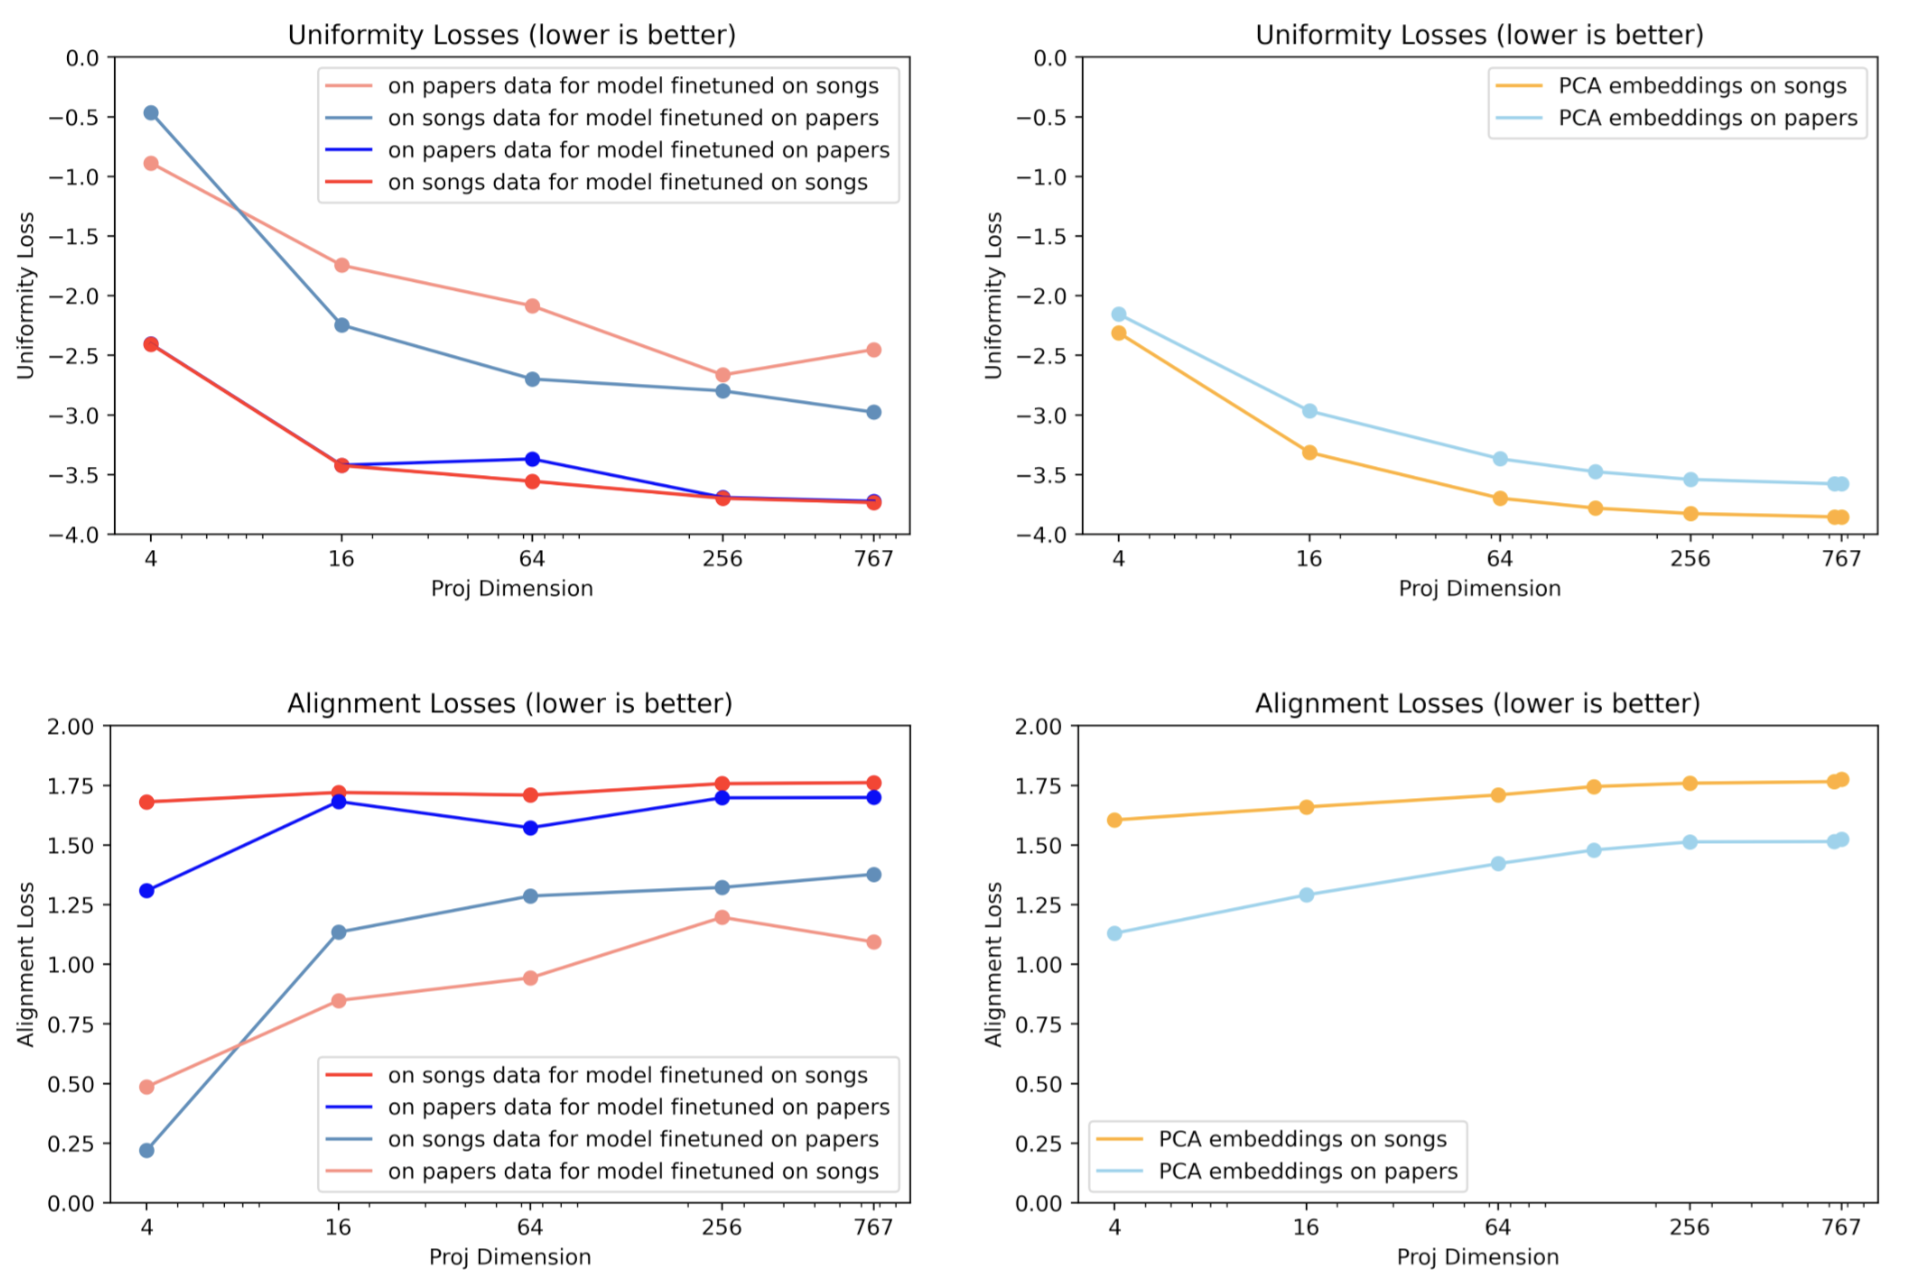
\includegraphics[width=1.0\linewidth]{Images/all_align_unif.png}
\caption{Uniformity and alignment losses.}
\label{fig:losses}
\end{figure}

\subsection{Songs and Papers Clusters Embedded with t-SNE}
Even with only 4 dimensions, the embeddings already separate lyrics from papers as two
distinct clusters (see Fig. \ref{fig:tsne}), indicating that coarse domain identity
survives aggressive compression. However, in 4D the clusters are elongated and less
compact, with visibly distorted shapes. At 16 dimensions, the clusters become rounder,
and local neighborhoods look more stable. This suggests that increasing dimensionality
from 4D to 16D does not create domain separation from scratch, but instead improves the
within-domain geometry: it reduces compression artifacts and yields a smoother manifold,
which is consistent with the concurrent improvement in STS-B performance.

\begin{figure}[h!]
\centering
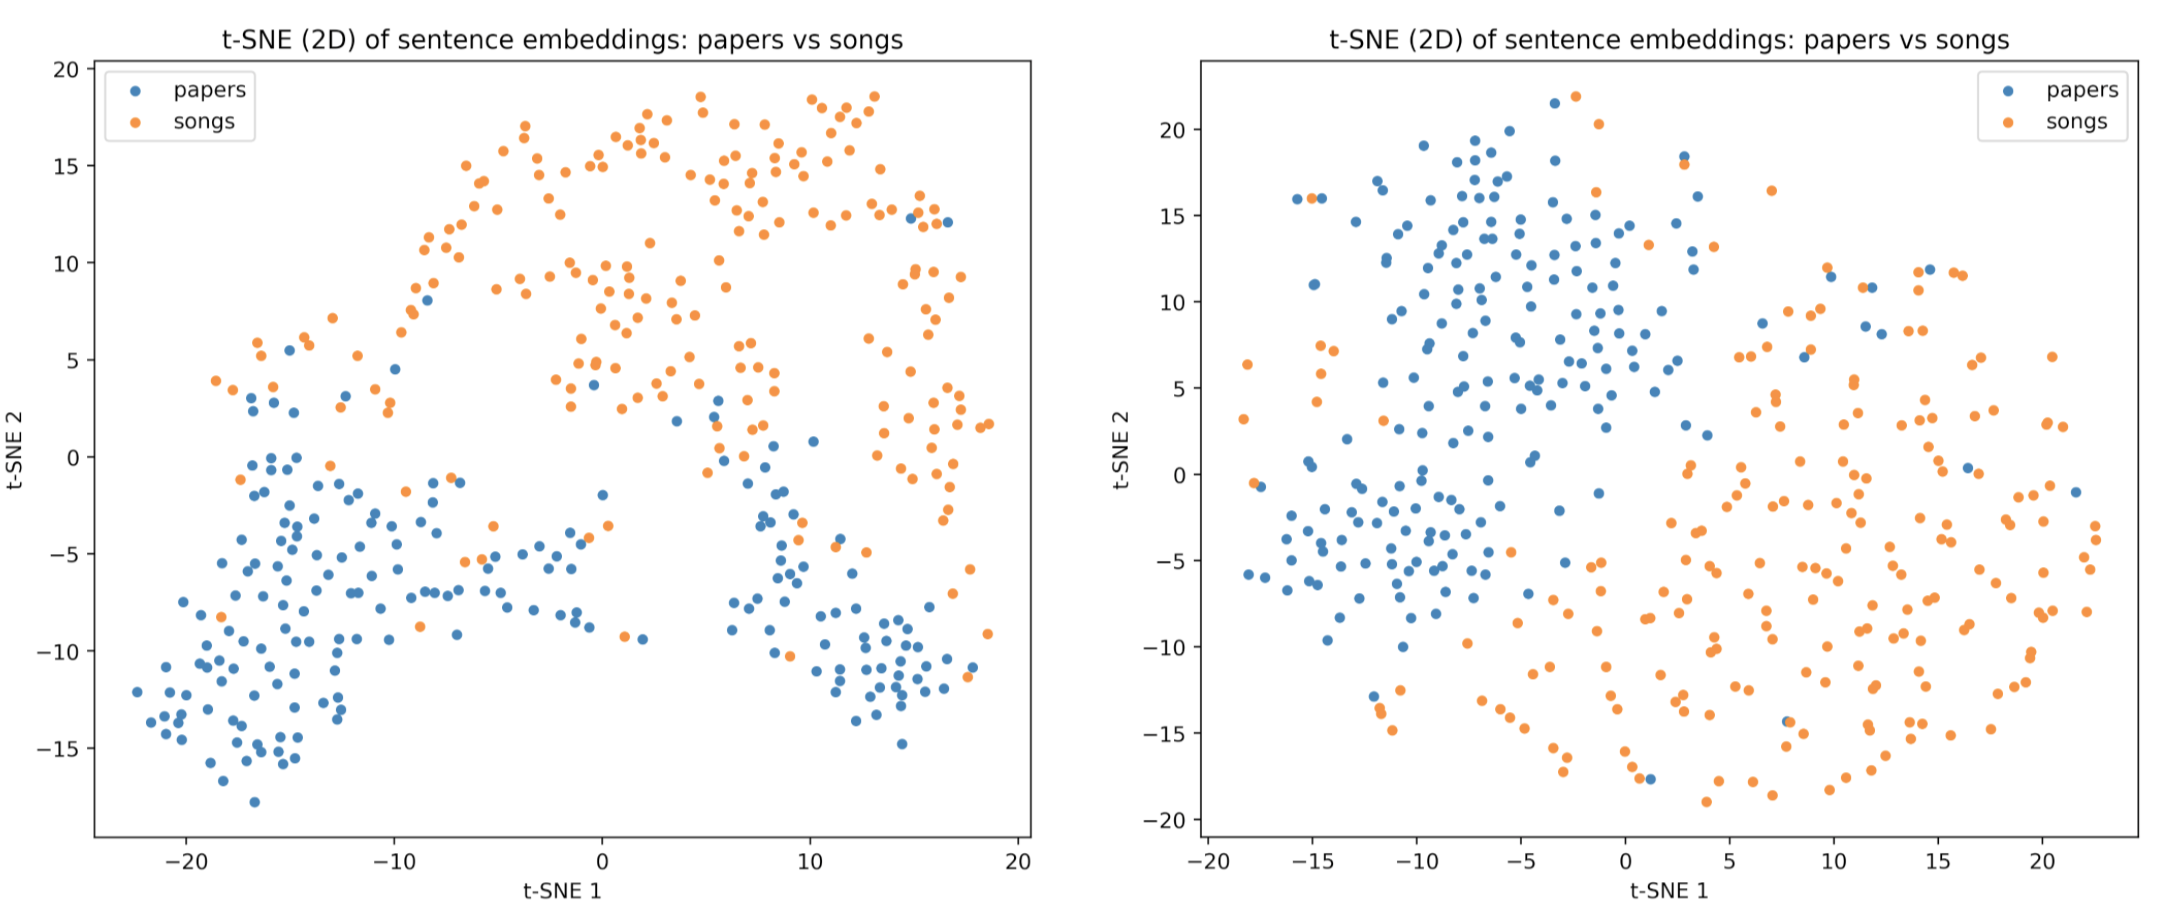
\includegraphics[width=1.0\linewidth]{Images/tsne_comp.png}
\caption{t-SNE results for 4D and 16D BERT+pooler models trained on songs.}
\label{fig:tsne}
\end{figure}

\subsection{Ablation on the Training Procedure}
For songs-trained models, with smaller dimensions (4, 16), the two-step training process
yields the best Spearman rank correlations, showing how \textbf{important the pooler is
for extreme dimensionality reduction} (see Fig. \ref{fig:ablation}). However, at certain
higher dimensions training only the encoder yields the best results. Training only the
pooler is not sufficient for learning useful representations for songs-based models.

For papers-based models, we see a similar trend, but the dimension cutoff at which the
pooler stops giving much benefit is higher, somewhere between 128D and 256D (again
hinting at the higher intrinsic dimensionality of scientific data). In addition, only
training the pooler with the frozen BERT backbone yields much better Spearman rank
results for papers-trained models than for songs-trained models -- perhaps hinting to us
that the frozen BERT encoder is initially better suited for academic text.

%/ replace with aksel's combined results for both songs and papers
\begin{figure}[h!]
\centering
\includegraphics[width=1.0\linewidth]{Images/ablation_2ax.png}
\caption{Ablation study on the two-step training procedure.}
\label{fig:ablation}
\end{figure}

\subsection{Challenges and Limitations}
We note that all reported results depend on a specific choice of backbone (BERT-base),
corpus size, and contrastive neighborhood definition. In addition, while STS-B Spearman
rank results provide an insightful semantic probe, it represents only one notion of
transfer learning performance.

\paragraph*{Evaluation Criteria} Selection of evaluation metrics (alignment, uniformity, STS-B Spearman rank)
was an area of much thought and discussion. Drawing inspiration from Gao et al. \cite{gao2021simcse}, we
explored enriching our unlabeled dataset with self-supervised positive pairs. We landed on sentence proximity
as a straightforward and effective method to generate these pairs without additional labeling.

\paragraph*{Contrasting Loss Finetuning} By design, the constrastive loss finetuning only seeks to optimize
local structure and better distribute embeddings along the unit hypersphere. However, the inherent upper
bound on this optimization objective comes from the pre-trained representations provided by BERT. Our
procedure is not designed to, nor is it likely to, drastically alter the global structure of the embedding
space. Hence, this route will not likely yield a dramatic improvement in sentence embedding, or revolutionize the field.

\paragraph*{Scope} Due to time and resource constraints, we limited out experiments to two esoteric domains
of the english language. A more comprehensive study would include a much broader array of domains,
self-labeling algorithms, and backbone architectures.

\paragraph*{BERT} As our backbone, BERT-base-uncased is a well-established model for sentence embeddings.
However, there are more recent encoder architectures (e.g., RoBERTa, DeBERTa, etc.) available for
exploration. In addition, the past five years have seen a preponderance of investment into closed-source LLMs
(e.g., GPT, Gemini, Grok, Claude, etc.) that may offer superior embedding capabilities (with the caveat that
it's uncertain that cleanly demarcated encoder-decoder patterns exist in said closed models).
\subsection{Future Directions}
For future work, we would like to explore \textbf{additional domains} (such as news, code
comments etc.), try other \textbf{embedding models beyond BERT}, use
\textbf{alternative training objectives} (for instance, non-contrastive methods), enrich the suite of
\textbf{evaluation methods}, and implement competing self-supervised \textbf{sentence pair labeling algorithms}.

Expanding the scope a bit, it would be interesting to move beyond all-purpose sentence embeddings and explore
\textbf{task-specific embeddings} and \textbf{multimodal embeddings}, modeling language in a
\textbf{hierarchical manner}, moving beyond euclidean spaces into \textbf{non-euclidean geometries}, and
exploring the notion of \textbf{intrinsic dimensionality}.

\section{Conclusion}

\subsection{Summary of Findings}
\begin{itemize}
\item \textbf{Lyrics-trained models dominate at low dimensions (4–256D) on STS-B}, while
papers-trained models only overtake at 768D $\Rightarrow$ \textbf{scientific text appears
inherently higher-dimensional}.
\item \textbf{Uniformity and alignment conflict} with each other, with
\textbf{papers-trained models being more stable} when transitioning from in-distribution
to out-of-distribution data.% TODO: this sentence doesn't sound coherent
\item \textbf{Low-dimensional embeddings} are able to \textbf{separate domains (even at
4D)}, but more meaningful local structure emerges only at 16D or more.
\item Linear compression \textbf{(PCA) is insufficient for transfer learning} tasks in
our experiments: contrastive learning is necessary to expose semantic structure even at
small dimensions. It is advised to retrain, instead of linearly transform dimensions, if
target dimensionality changes.
\end{itemize}

\subsection{Contributions of each team member}
\begin{itemize}
\item \textbf{A.C.}: BERT+pooler architecture implementation, BERT+PCA architecture
implementation and evaluation on 4-767D, partial report write-up. % preprocessing?
\item \textbf{A.K-W.}: Data collection and preprocessing for both datasets, ablation
studies on the BERT+pooler architecture for both datasets with training and evaluation on
4-767D, partial report write-up.
\item \textbf{M.G.}: Initial literature review, evaluation suite and graphics
implementation, baseline BERT+pooler training and evaluation on 4-767D for both datasets,
poster preparation, partial report write-up.
\end{itemize}

\section*{Acknowledgments}
We are grateful to Prof. Nakul Verma, and our teaching assistants, Noah Bergam and Szymon
Snoeck, for their feedback on our ideas.

\section*{Code Availability}
All our code can be found at \hyperlink{Github}{https://github.com/AlenaResiko/UML}.

\bibliographystyle{plainnat}
\bibliography{references}

\raggedbottom

\section*{Appendix}

\raggedbottom

\end{document}
